\chapter{Creación de webs en AWS y Azure}
La funcionalidad principal de estos servicios es el desarrollo de sitios webs o servicios web auto-escalables. Ambos ofrecen almacenamiento de ficheros y datos, aunque nosotros nos centraremos únicamente en la temática orientada a servicios web, ya que es el pilar de los dispositivos IoT o de los backend de las aplicaciones móviles actuales. 

La ventaja de utilizar la nube frente a proveedores de hosting es la fiabilidad y el escalado, mientras que en un proveedor estándar tendríamos que realizar llamadas a servicio técnico para poder escalar, en estas plataformas los servicios web se auto-escalan en función de la carga de trabajo que deben de ejecutar. Esto incluye reducir la capacidad en casos en los que el servicio no requiera tantos recursos y así no tener que ceñirnos a ningún plan.

\section{Servicios Web}
Los servicios web son aplicaciones que proveen de información a una o varias aplicaciones por medio de distintos protocolos. Principalmente destacan dos SOAP y REST, veamos una pequeña introducción a estos protocolos.

\subsection{SOAP}
Simple Object Access Protocol, es un estándar que utiliza XML para transmitir la información, a su vez utiliza distintos componentes para informar de cómo se utiliza el servicio (WSDL) y de transmitir a los servidores qué servicios dispone un servidor concreto (UDDI). Excesivamente verboso, está en proceso de ser reemplazado por REST.

\subsection{REST}
Representation State Transfer, protocolo que utiliza HTTP para transferir el estado de los datos entre el servidor y el cliente. A diferencia de SOAP que hay que realizar una ruta distinta para manipular los datos, se aprovecha de los métodos HTTP para decidir que hacer con un dato en concreto utilizando la misma ruta.

\section{Creación de una web en AWS}
AWS es una plataforma que lleva implícito en su nombre el proporcionar servicios webs (Amazon Web Services). Amazon ofrece una serie de recursos para crear sitios y servicios webs. Desgraciadamente, el plan de estudiante no dispone de acceso a la plataforma principal que permita crear un sitio web y no podemos poner un ejemplo como sí hemos podido hacer en el resto de apartados

Amazon dispone de los siguientes principales para la construcción de sitios y servicios webs:
\begin{itemize}
	\item \textbf{Amazon EC3:} Se encarga de ejecutar el servidor web y las tareas de procesamiento.
	\item \textbf{Amazon S3:} Permite almacenar ficheros y ser accesibles por el servidor web.
	\item \textbf{Amazon RDS:} Sistema de gestión de bases de datos.
\end{itemize}

\begin{figure}[h]
	\centering
	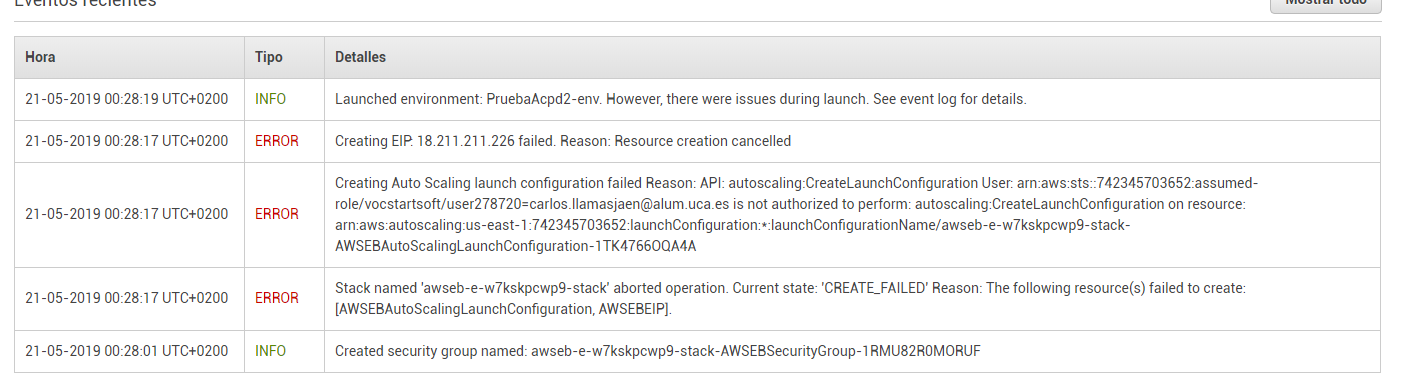
\includegraphics[scale=0.45]{ImagenesAWS/Web/error_aws.png}
	\caption{Error al crear un entorno en Amazon Elastic Beanstalk}
	\label{AWSWEB1}
\end{figure}

\section{Creación de una web en Azure}
En Azure sí que hemos podido desarrollar una sencilla web. La ventaja fundamental de Azure frente a AWS es que permite a través de Visual Studio publicar un sitio o servicio web con tal de hacer un click, lo que permite un desarrollo bastante más rápido que utilizar AWS. En Azure disponemos de los principales lenguajes para desarrollar aplicaciones o servicios web, en este ejemplo vamos a crear una simple página html que modificaremos en la presentación para demostrar la sencillez que tiene la integración con Visual Studio.

En Azure los sitios webs se denominan App Services, pese a que es posible desarrollar un sitio web, están más orientados a implementar un servicio web.

\newpage
El primer paso es seleccionar el plan, aprovecharemos las horas gratuitas que disponemos. Tenemos que seleccionar el dominio, el cúal podemos utilizar de los que Azure proporciona de forma gratuita.

\begin{figure}[h]
	\centering
	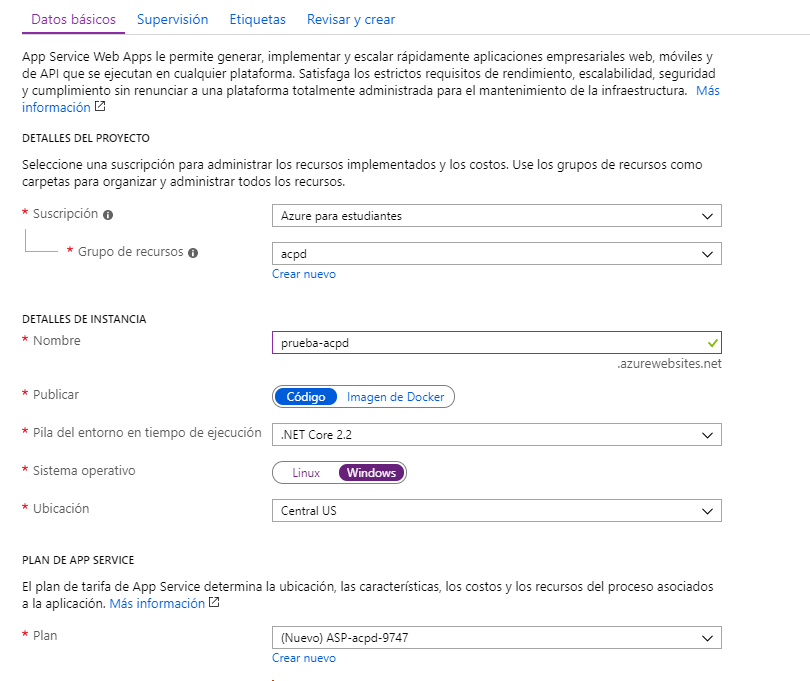
\includegraphics[scale=0.55]{web_azure/creacion1.png}
	\caption{Creación del sitio web}
	\label{AZWEB1}
\end{figure}

Una vez seleccionado el plan se nos pide seleccionar si queremos métricas, que hemos desactivado ya que son de pago. En el siguiente paso se nos pide si queremos asignar etiquetas de facturación al recurso.

\begin{figure}[h]
	\centering
	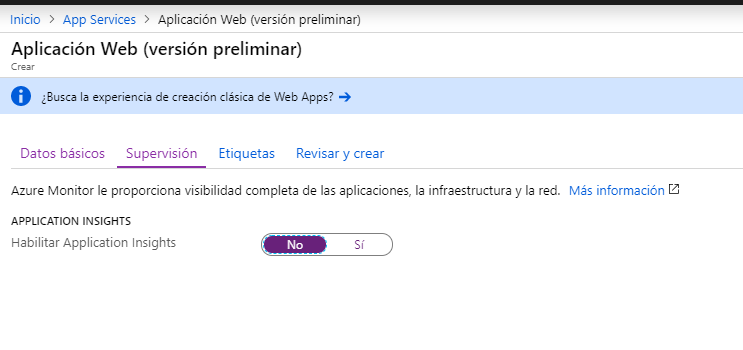
\includegraphics[scale=0.55]{web_azure/creacion2.png}
	\caption{Selección de métricas}
	\label{AZWEB2}
\end{figure}

\newpage
\begin{figure}[h]
	\centering
	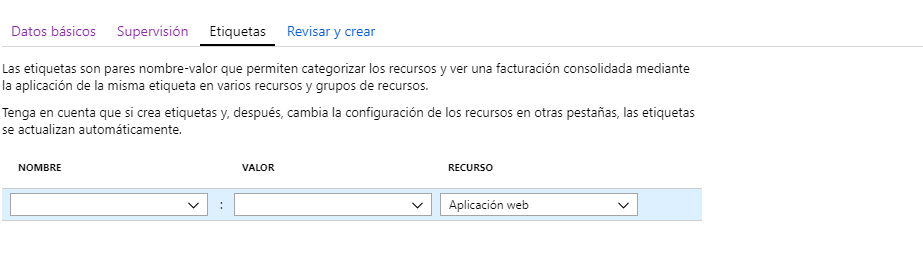
\includegraphics[scale=0.55]{web_azure/creacion3.png}
	\caption{Selección de etiquetas}
	\label{AZWEB3}
\end{figure}

Una vez hecho esto tenemos el sitio ya arrancado, pese a que muestra una página de demostración.

\begin{figure}[h]
	\centering
	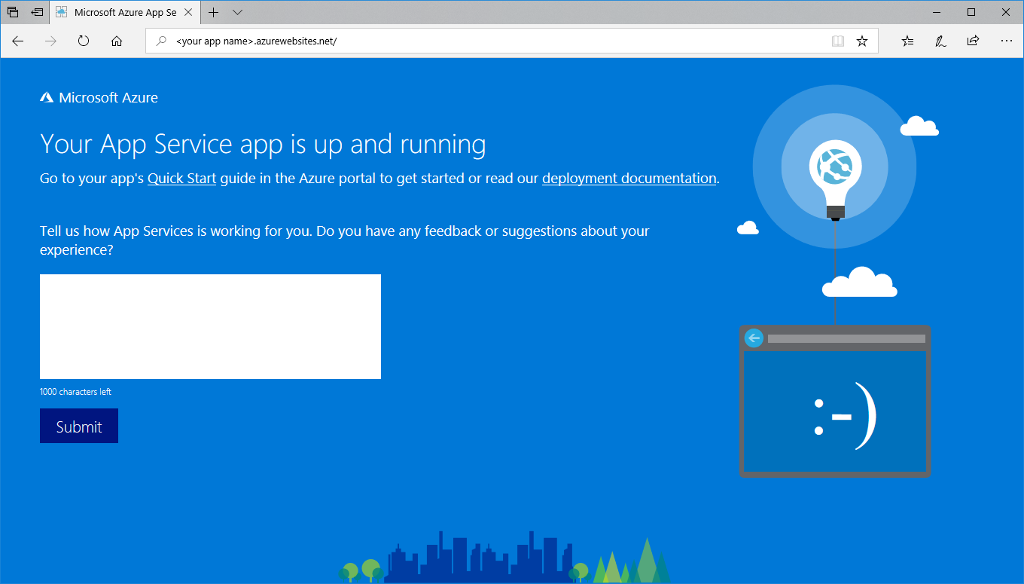
\includegraphics[scale=0.4]{web_azure/web1.png}
	\caption{Página de demostración}
	\label{AZWEB4}
\end{figure}

\newpage
Ahora pasaremos a subir una página desde Visual Studio. Para ello es necesario descargar el perfil de publicación, para poder subir el sitio al servidor.

\begin{figure}[h]
	\centering
	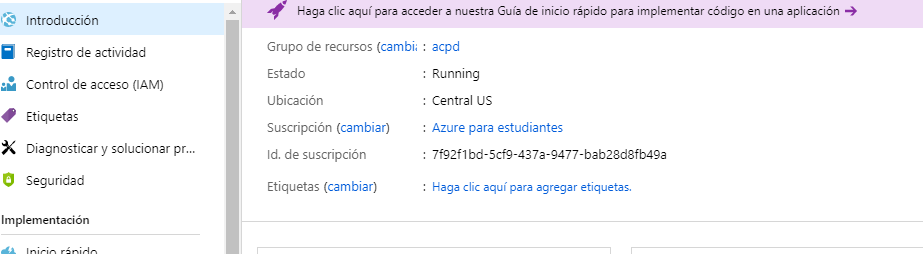
\includegraphics[scale=0.55]{web_azure/centro.png}
	\caption{Centro de control del sitio web}
	\label{AZWEB5}
\end{figure}

El código de la web es muy simple, únicamente imprime un código HTML con una foto y un texto.

\begin{figure}[h]
	\centering
	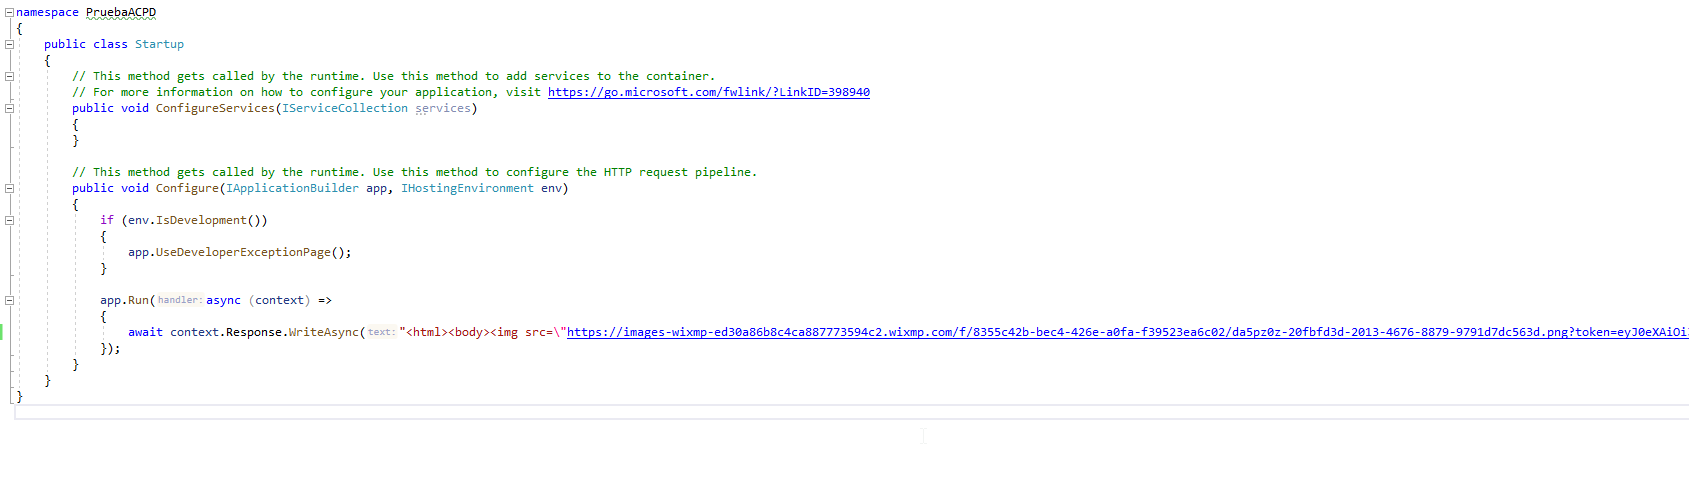
\includegraphics[scale=0.3]{web_azure/web2.png}
	\caption{Código fuente}
	\label{AZWEB6}
\end{figure}

Finalmente seleccionamos publicar en el explorador de soluciones y cargamos el perfil de publicación. Solamente tenemos que hacer click en publicar, para que el sitio se suba a Azure.

\begin{figure}[h]
	\centering
	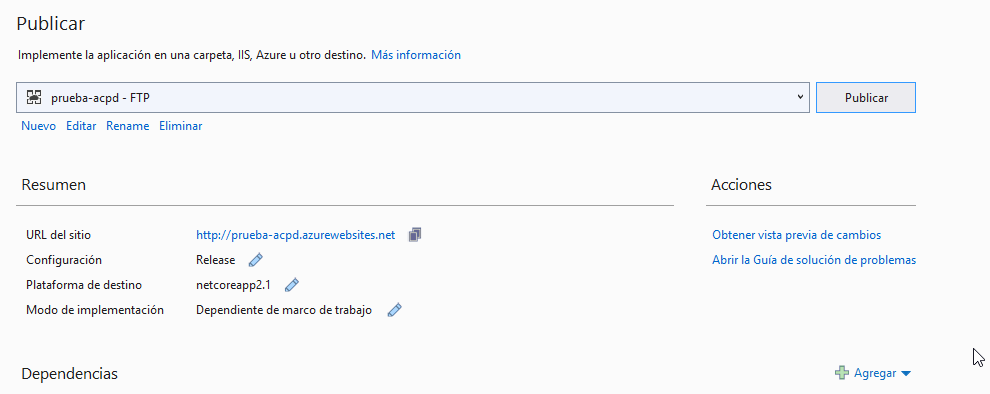
\includegraphics[scale=0.55]{web_azure/web3.png}
	\caption{Publicación de sitio web}
	\label{AZWE7}
\end{figure}

\newpage
\begin{figure}[h]
	\centering
	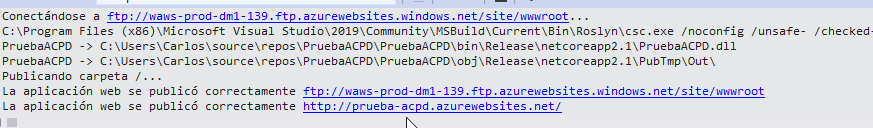
\includegraphics[scale=0.55]{web_azure/web4.png}
	\caption{Publicación correcta}
	\label{AZWEB8}
\end{figure}

Cargamos el sitio web y podemos ver que ha cambiado

\begin{figure}[h]
	\centering
	
\includegraphics[scale=0.55]{web_azure/web5.png}
	\caption{Web una vez subida}
	\label{AZWEB9}
\end{figure}

Con esto ya tendríamos listo el sito web, obviamente este es un ejemplo sencillo, un ejemplo más complejo lo tenemos en la página web smallpdf.com, es una página web que realiza diversas tareas de manipulación sobre ficheros PDF y que utiliza la nube de AWS para procesar y almacenar temporalmente los archivos PDF ya manipulados.


